\documentclass{article}
\usepackage{graphicx, color, multicol}


\setlength{\textwidth}{6.5in}
\setlength{\textheight}{8.0in}
\setlength{\oddsidemargin}{0in}
\setlength{\evensidemargin}{0in}
\setlength{\parskip}{2ex}
\setlength{\parindent}{0in}


\begin{document}
%To display answers, replace "white" with "red".
\newcommand{\answer}[1]{\color{red}#1}

\pagestyle{myheadings}\markright{
CU Boulder \hspace{0.5in} MATH 2510 - Introduction to Statistics }

\begin{center}
\textbf{\underbar{In-class Worksheet 25}}
\end{center}

\begin{enumerate}

%Section 10.2 #3
\item Explain why ``goodness-of-fit'' tests are always right-tailed tests. 

{\answer
The formula for computing $\chi^2$ is $ \chi^2 = \sum \frac{(O-E)^2}{E}$.  So, the larger the difference between the {\em Observed} frequencies and the {\em Expected} frequencies, the greater the $\chi^2$ value.  The greater the $\chi^2$ value, the further out on the right-tail the test statistic lies.  Also, the greater $\chi^2$ values lead to the conclusion that the differences are too great to be explained by chance alone, or, in other words, the evidence indicates that the population follows a different distribution that the {\em Expected} distribution.
}


%Section 10.2 #16	
\item A gambler complained about the dice.  They seemed to be loaded!  The dice were taken off the table and tested one at a time.  One die was rolled 300 times and the following frequencies were recorded. \\
\begin{tabular}{l||rrrrrr}
\hline
Outcome & 1 & 2 & 3 & 4 & 5 & 6 \\
\hline
&&&&&& \\
Observed Frequency $O$ &  62 & 45 & 63 & 32 & 47 & 51 \\
&&&&&& \\
\hline
&&&&&& \\
Expected Frequency $E$ &\hspace{0.5cm}{\answer 50} &\hspace{0.5cm}{\answer 50} &\hspace{0.5cm}{\answer 50} &\hspace{0.5cm}{\answer 50} &\hspace{0.5cm}{\answer 50} &\hspace{0.5cm}{\answer 50}  \\
&&&&&& \\
\hline
\end{tabular}

Do these data indicate the the die is unbalanced?  Use a 1\% level of significance.

	\begin{enumerate}
	%
	\item Enter the expected number of rolls out of 300 for a balanced (fair) die in the table above.
	\item State the null and alternate hypotheses for the desired test. 
	
	{\answer 
	$H_0$: The distributions are the same. \\ $H_1$: The distributions are not the same.
	} 
	
	\item What are the degrees of freedom? 
	
	{\answer 
	$d.f. = 6-1 = 5$
	} 
	
	\item What is the $P$-value?  
	
	{\answer 
	Using \texttt{$\chi^2$GOF-Test} with $L_1$ as the observed frequencies and $L_2$ as the expected frequencies with $d.f. = 5$, $P=0.0195865323$.
	} 

	\item What is the conclusion of the test and what does this mean in terms of the fairness of the die? 
	
	{\answer 
	Because $P > \alpha$, we do not reject $H_0$.  So, at the 1\% level of significance, there is insufficient evidence to support the claim that the die is not fair.
	} 
	
	%
	\end{enumerate}
	
\vfill
\pagebreak

%Section 10.2, #10
\item Let $x$ be a random variable that represents the average daily temperature (in $^\circ F$) in January for the town of Hana, Maui.  The $x$ variable has a mean $\mu = 68^\circ F$ and a standard deviation $\sigma = 4^\circ F$.  A 20-year study (620 January days) gave the entries in the rightmost column of the following table. 

\begin{tabular}{l||c||c||c}
Region under normal curve & $x\ ^\circ F$ & Expect \% from normal curve & Observed number of days \\
\hline \hline
$\mu -3\sigma \leq x < \mu - 2\sigma$ & $56 \leq x < 60$ & 2.35\% & 14 \\
\hline
$\mu -2\sigma \leq x < \mu - \sigma$ & $60 \leq x < 64$ & 13.5\% & 86 \\
\hline
$\mu -\sigma \leq x < \mu $ & $64 \leq x < 68$ & 34\% & 207 \\
\hline
$\mu \leq x < \mu + \sigma$ & $68 \leq x < 72$ & 34\% & 215 \\
\hline
$\mu +\sigma \leq x < \mu + 2\sigma$ & $72 \leq x < 76$ & 13.5\% & 83 \\
\hline
$\mu +2\sigma \leq x < \mu + 3\sigma$ & $76 \leq x < 80$ & 2.35\% & 15 \\
\hline
\end{tabular}

Use a 1\% level of significance to test the claim that the average daily temperature follows a normal distribution with $\mu = 68$ and $\sigma = 4$.

	\begin{enumerate}
	%
	\item State the null and alternate hypotheses. 
	
	{\answer 
	$H_0$: The average daily temperature fits the normal distribution. 
	
	$H_1$: The average daily temperature does not fit the normal distribution. 
	} 
	
	\item Explain why the values in the ``expected" column are consistent with a normal distribution. 
	
	{\answer 
	The graph of the normal curve shown here describes where the values in the column come from.}
	%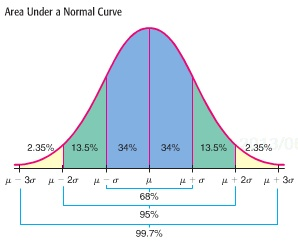
\includegraphics[scale=0.3]{WS10_NormalArea.jpg}  %**Use for answer key in place of space
	\vspace{2cm}
	
	\item What are the degrees of freedom? 
	
	{\answer 
	$d.f.=6-1 = 5$
	} 
	
	\item What is the $P$-value? 
	
	{\answer 
	Using \texttt{$\chi^2$GOF-Test} with $L_1$ as the observed number of days and $L_2$ as the expected number of days with $d.f. = 5$, $P=0.9983862518$.
	} 
	
	\item What is the conclusion of the test and what does this mean in terms of the distribution of daily January temperatures? 
	
	{\answer 
	Because $P > \alpha$, we do not reject $H_0$.  So, at the 1\% level of significance, there is insufficient evidence to support the claim that the distribution of daily temperatures does not fit a normal distribution.
	} 
	
	%
	\end{enumerate}
	
\end{enumerate}
\vfill

\end{document}

